\section{Algorithm Design}
In this section, we wil talk about the desing of the algorithms.
\subsection{Feature Design}
The problem can be simplified to a binary classification problem.
The input is the features of the data sets, and the output is the winner side (the sentinel or the scourge).
The prediction will be conducted before the game.
So available features include hero lineup, hero combination, game time and the game results.
Therefore, features include three parts: 
\begin{enumerate}
\item Hero Lineup (111 * 2 dimensions): There are 111 heroes in the game.
Each team will pick 5 heroes in each game.
Each feature can be 1 or 0, meaning picked or not picked.
Therefore, there are 222 dimensions for hero presentation.
\item Positive Relationship (30 * 2 dimenstions):
In Dota, some heroes can cooperate with each other to increase the attack output.
For example, the hero Ursa and the hero Io are always picked together in the same team.
They can cooperate with each other and give a very high attack output.
We choose the most influential pairs of heroes (30 pairs) for each team in positive relationship.
\item Negative Relationship (30 * 2 dimenstions):
In Dota, some heroes's performance are lower by some other heroes.
When they are in the different teams, one hero always push much pressure on the other hero in the other team.
We choose the most importnat pairs of heroes (30 pairs) for each team in negative relationship.
\item Time (1 dimension):
This feature is used to show how long the game lasts.
\item The Result (1 dimension): 0 or 1, Team A wins or Team B wins.
\end{enumerate}
\subsection{Algorithm Decision}

After attempts of several algorithms, such as Decision Tree, Logistic Regression, Natural Network and SVM, we select Decision Tree as our model.
 

XXX: We need more descriptions why we choose decision tree.


Decision Tree is a tree-like model of decisions to analyze problems.
 The nature of a decision three is decision rules.
 A decision tree about discount is presented in Figure~\ref{fig:ctree}.


\begin{figure}[!htbp]
\centering
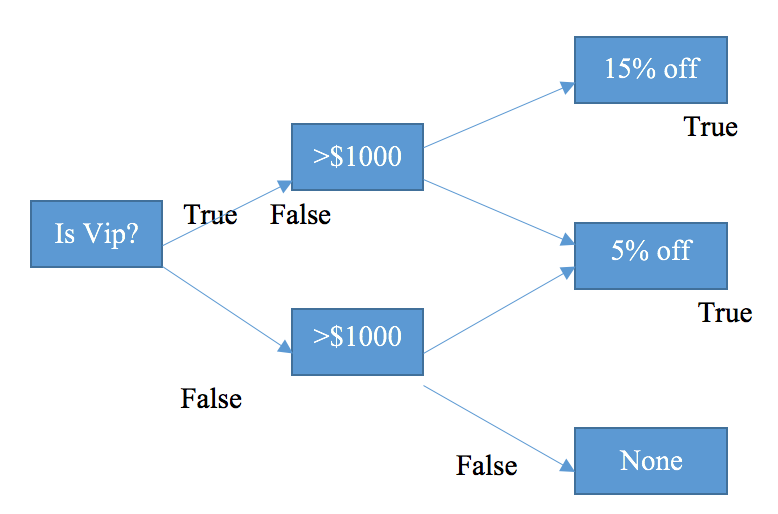
\includegraphics[width=8.0cm]{ctree.png} 
\newline
\caption{An Example of C4.
5 Decision Tree}
\label{fig:ctree} 
\end{figure}

We adopt C4.
5 to generate a decision tree for the problem.
 The algorithm is proposed by Ross Quinlan~\cite{quinlan}, which is an extension of his earlier ID3 algorithm.

The pseudocode~\cite{Kotsiantis} of the general algorithm for building decision trees by C4.
5 is: 

\begin{enumerate}
\item Check for base cases.

\item For each attribute a, find the normalized information gain ratio from splitting on a.

\item Let a\_best be the attribute with the highest normalized information gain.

\item Create a decision node that splits on a\_best.

\item Recur on the sublists obtained by splitting on a\_best, and add those nodes as the children of the node.

\end{enumerate}


